%---------------------------------------------------------%
%______//------             GAC             ------\\______%
%______||------         Chapitre 0          ------||______%
%______\\------         Motivations         ------//______%
%---------------------------------------------------------%

\chapter{Motivations}

  %Déf 0.1
  \begin{defi}
    Soit $G$ un groupe muni d'une loi ``$\cdot$''. $G$ est un \emph{groupe} si 
    \begin{enumerate}
    \item il existe un élément neutre $e \in G$;
    \item pour chaque élément $g \in G$, il existe un inverse $g^{-1}$;
    \item $\cdot$ est associative: $(x\cdot y)\cdot z = x \cdot (y \cdot z)$.
    \end{enumerate}
  \end{defi}

  \begin{exs}
    \begin{enumerate}
    \item $G = \{e\}$.
    \item $G = (\Z, +)$.
    \item $G = \Z/n\Z$.
    \item $G = S_3$ le groupe des symétries d'un triangle.
    \item $G = D_4$ le groupe des symétries d'un carré.
    \end{enumerate}
  \end{exs}

  \section{Algorithmes et combinatoire?}

    Chaque groupe $G$ admet un présentation 
      \[G = \langle X | R \rangle \]
    où $X \subset G$ est une partie génératrice et $R$ est un ensemble de relations.

    \begin{exs}
      \begin{enumerate}
      \item $\Z = \langle a = 1 | - \rangle$.
      \item $S_3 = \langle t_1, t_2 | t_1^2 = e = t_2^2, (t_1t_2)^3 = e\rangle$.
      \item $D_4 = \langle x, y | x^2 = y^4 = (xy)^2 = e \rangle$.
      \item $\Z/7\Z = \langle x | x^7 = e\rangle$.
      \end{enumerate}
    \end{exs}
    
    Attention: la présentation n'est pas unique, car par exemple $\Z = \langle a, b | b = 1 \rangle$.

  \section{Problèmes de Dehn}

    \subsection{Problème de l'égalite (PE)}

      Existe-t-il un algorithme permettant de décider pour tout couple de mots $(u,v)$ sur $X$ (pour un groupe
      $G = \langle X | R \rangle$) s'ils représentent le même élément du groupe ($u =_G v$)?

      Par exemple, soit $G = \langle x,y,z |  x^2yx^{-1}z = x^3y^3\rangle$. Est-ce que $xyx^{-1}z =_G
      zx^2y^{-1}z$? Ou par exemple dans $S_3$, est-ce que $t_1t_2t_1^3t_2 =_{S_3} t_2t_1$? En fait, oui car
      \begin{align*}
        t_1t_2t_1^3t_2 &= t_1t_2t_1t_1^2t_2 & t_1^2 = e\\
        &= t_1t_2t_1t_2 & (t_1t_2)^3 = e\\
        &= t_2^{-1}t_1{-1} & t_1 = t_1^{-1},\ t_2 = t_2^{-1}\\
        &= t_2t_1.
      \end{align*}

    \subsection{Problème des mots (PM)}

      Existe-t-il un algorithme permettant de décider pour tout mot $w$ sur $X$ si $w =_G e$?

      Si $G = \langle X | R \rangle$, on peut dessiner son graphe de Cayley, qui est un espace métrique. Les
      sommets de ce graphe sont $\{g \in G\}$ et les arêtes sont $\{(g, gx)\, :\, g \in G,\, x \in X\}$.

      \begin{exs}
        \begin{enumerate}
        \item Considérons par exemple 
            \[S_3 = \{e, (12) = t_1, (23) = t_2, (13) = t_3, (123)=t_4, (132) = t_5\}.\]
          On a $X = \{t_1, t_2\}$. Le graphe de Cayley est
          \begin{center}
            \begin{tikzpicture}
              \draw (0,0) node[scale=0.8]{$\bullet$} node[above right]{$t_4$};
              \draw (4,-3) node[scale=0.8]{$\bullet$} node[right]{$t_3 = t_5t_2$};
              \draw (3,-2) node[scale=0.8]{$\bullet$} node[below left]{$t_5$};
              \draw (-4,-3) node[scale=0.8]{$\bullet$} node[below left]{$t_2$};
              \draw (-3,-2) node[scale=0.8]{$\bullet$} node[above left]{$e$};
              \draw (0,1) node[scale=0.8]{$\bullet$} node[right]{$t_1 = t_4t_2$};
              \draw[color = OliveGreen] (0,1) -- (0,0);
              \draw[color = OliveGreen] (4,-3) -- (3,-2);
              \draw[color = OliveGreen] (-4,-3) -- (-3,-2);
              \draw[color = red] (0,0) to[bend left] (4,-3);
              \draw[color = red] (3,-2) to[bend left] (-4,-3);
              \draw[color = red] (-3,-2) to[bend left] (0,1);
            \end{tikzpicture}
          \end{center}

        \item Considérons $\Z = \langle 2, 3 | 2+2+2 = 3+3\rangle$. Dessinons son graphe de Cayley.
          \begin{center}
    
            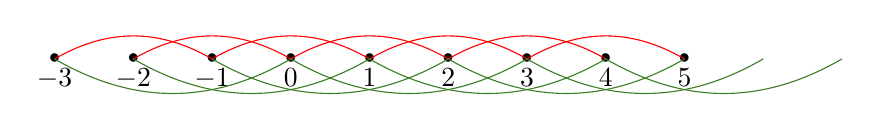
\begin{tikzpicture}
              \foreach \k in {-3,-2,...,5} { \draw (\k, 0) node[scale=0.8]{$\bullet$} node[below]{$\k$}; }
              \foreach \k in {-3, -2, ..., 3}{ \draw[color = red] (\k, 0) to[bend left] ({\k+2}, 0); }
              \foreach \k in {-3, -2, ..., 4}{ \draw[color = OliveGreen] (\k, 0) to[bend right] ({\k+3}, 0); }
            \end{tikzpicture}

          \end{center}
          En fait on dit que ce groupe est quasi-isométrique à $\Z = \langle 1 | - \rangle$.
        \end{enumerate}
      \end{exs}



  




%%% Local Variables:
%%% mode: latex
%%% TeX-master: "../GAC_cours.tex" 
%%% End: